\section{Time step methods}

We can now turn our attention to numerical methods for conservation laws.
For that we will begin with the scalar advection equation
\begin{align*}
	\partial_t u + a\partial_x u &= 0, \quad \text{in }\R \times \parentheses*{0, \infty},\\
	u\parentheses*{x, 0} &= u_0\parentheses*{x}, \quad \text{in }\R
\end{align*}
with advection speed \(a \in \R\).
The techniques developed for this simple problem will be generalized later.


\subsection{Discretization and update rule}

\begin{definition}[Advection discretization]
	\begin{enumerate}
		\item The \(\parentheses*{x, t}\)-domain will be discretized by an equidistant grid \(\mathcal{T}\) with \emph{spatial step size} \(\Delta x\) and \emph{temporal step size} \(\Delta t\) with \(\frac{\Delta x}{\Delta t} = \text{const.}\) (also for \(\Delta x, \Delta t \to 0\)).
		We consider \emph{spatial grid points} and \emph{time points} (or time levels) as
		\[
			x_j = j\Delta x \quad \parentheses*{j \in Z}, \quad \text{and} \quad t_n = n\Delta t \quad \parentheses*{n = 0, 1, \ldots},
		\]
		respectively.
		Furthermore, for \(j \in \Z\) we consider \emph{grid cells} \(\brackets*{x_{j - \frac{1}{2}}, x_{j + \frac{1}{2}}}\) with \(x_{j \pm \frac{1}{2}} = x_j \pm \frac{1}{2}\Delta x\).
		\item For the discretization of the solution \(u: \R \times \R^+ \to \R\) at time point \(t_n\), we consider either \emph{point values}
		\[
			u_j^n := u\parentheses*{x_j, t_n}
		\]
		or \emph{cell mean values}
		\[
			\bar{u}_j^n := \frac{1}{\Delta x}\int_{x_{j - \frac{1}{2}}}^{x_{j + \frac{1}{2}}}u\parentheses*{x, t_n}\d x
		\]
		for \(j \in \Z\).
	\end{enumerate}
\end{definition}

\begin{remark}
	\begin{enumerate}
		\item A pointwise discretization using point values shares similarities to the discretization in finite difference methods.
		However, cell mean values will become more appropiate for conservation laws, as we will see later.
		\item We sometimes consider spatially periodic solutions with period \(L > 0\) so that
		\[
			u\parentheses*{x, t} = u\parentheses*{x + L, t} \quad \forall x \in \R
		\]
		for all \(t \ge 0\).
		In that case we only discretize one period with \(N\) points \(u_j^n, j = 1, \ldots, N\).
		\item The \(N\)-dimensional vectors
		\[
			u_{\Delta x}^n = \begin{pmatrix}
				u_1^n\\
				\vdots\\
				u_N^n
			\end{pmatrix} \quad \text{and} \quad \bar{u}_{\Delta x}^n = \begin{pmatrix}
				\bar{u}_1^n\\
				\vdots\\
				\bar{u}_N^n
			\end{pmatrix}
		\]
		will be used to collect the numerical unknowns on one time level \(n\).
		\item For an arbitrary point \(\parentheses*{x, t} \in \R \times \R^+\) we will use the piecewise constant \emph{grid function} \(u_{\Delta t}\) given by
		\[
			u_{\Delta t}\parentheses*{x, t} = u_j^n, \quad \text{if }\parentheses*{x, t} \in \brackets*{x_{j - \frac{1}{2}}, x_{j + \frac{1}{2}}} \times \left[t_n, t_{n + 1}\right),
		\]
		which provides a function approximation of \(u\) in \(\R \times \R^+\) based on grid point values.
		Similarly for cell mean values of course.
	\end{enumerate}
\end{remark}

\begin{definition}[Time step method]
	We will write a (one step) \emph{time step method} by using an \emph{update rule} \(H_{\Delta t}\) of the form
	\[
		u_{\Delta x}^{n + 1} = H_{\Delta t}\parentheses*{u_{\Delta x}^n} \quad \text{or} \quad u_j^{n + 1} = H_{\Delta t}\parentheses*{u_{\Delta x}^n; j}.
	\]
	If \(H_{\Delta t}\) is applied to a function \(v: \R \to \R\), we define \(H_{\Delta t}\parentheses*{v}\) such that \(v\) will be evaluated at grid points.
	The result of \(H_{\Delta t}\) can be interpreted as a grid function such that the evaluation \(\brackets*{H_{\Delta t}\parentheses*{v}}\parentheses*{x}\) makes sense.
\end{definition}

\begin{remark}
	\begin{enumerate}
		\item Starting from a discretized initial condition
		\[
			u_j^0 = u_0\parentheses*{x_j}, \quad j \in \Z,
		\]
		we proceed step-wise from time level \(t_n\) to time level \(t_{n + 1}\), that is
		\[
			u_j^1 = H_{\Delta t}\parentheses*{u_{\Delta x}^0; j}, \quad u_j^2 = H_{\Delta t}\parentheses*{u_{\Delta x}^1; j}, \quad \text{etc.}
		\]
		\item The update rule may depend on \(\Delta x\) and \(\Delta t\) and parameters of the equation.
	\end{enumerate}
\end{remark}


\subsection{Some simple methods}

We will list a variety of existing ideas to discretize the advection equation:
\begin{enumerate}
	\item Using one-sided, forward, finite differences we can derive an approximation via
	\[
		\partial_t u + a\partial_x u = 0 \implies \frac{u_j^{n + 1} - u_j^n}{\Delta t} + a\frac{u_{j + 1}^n - u_j^n}{\Delta x} = 0.
	\]
	The discretized equation can be solved for \(u_j^{n + 1}\), which yields
	\[
		u_j^{n + 1} = u_j^n + \frac{a\Delta t}{\Delta x}\parentheses*{u_j^n - u_{j + 1}^n} =: H_{\Delta t}\parentheses*{u_{\Delta x}^n; j}.
	\]
	As stencil we have
	\begin{center}
		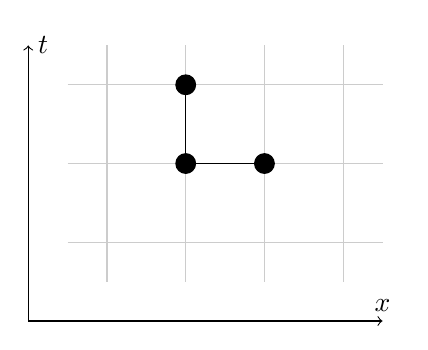
\begin{tikzpicture}
			\draw[<->] (0,3.5) node[right] {\(t\)} -- (0,0) -- (4.5,0) node[above] {\(x\)};
			\draw[white!80!black] (1,0.5) -- (1,3.5);
			\draw[white!80!black] (2,0.5) -- (2,3.5);
			\draw[white!80!black] (3,0.5) -- (3,3.5);
			\draw[white!80!black] (4,0.5) -- (4,3.5);
			\draw[white!80!black] (0.5,1) -- (4.5,1);
			\draw[white!80!black] (0.5,2) -- (4.5,2);
			\draw[white!80!black] (0.5,3) -- (4.5,3);
			\filldraw (2,3) circle (.125);
			\filldraw (2,2) circle (.125);
			\filldraw (3,2) circle (.125);
			\draw (2,3) -- (2,2) -- (3,2);
		\end{tikzpicture}
	\end{center}
	\item Instead of the simple one-sided formula, we could use central differences:
	\[
		\partial_x u \approx \frac{u_{j + 1}^n - u_{j - 1}^n}{2\Delta x} \implies u_j^{n + 1} = u_j^n + \frac{a\Delta t}{2\Delta x}\parentheses*{u_{j - 1}^n - u_{j + 1}^n}.
	\]
	As stencil we then obtain
	\begin{center}
		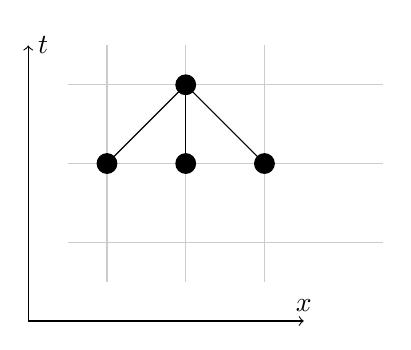
\begin{tikzpicture}
			\draw[<->] (0,3.5) node[right] {\(t\)} -- (0,0) -- (3.5,0) node[above] {\(x\)};
			\draw[white!80!black] (1,0.5) -- (1,3.5);
			\draw[white!80!black] (2,0.5) -- (2,3.5);
			\draw[white!80!black] (3,0.5) -- (3,3.5);
			\draw[white!80!black] (0.5,1) -- (4.5,1);
			\draw[white!80!black] (0.5,2) -- (4.5,2);
			\draw[white!80!black] (0.5,3) -- (4.5,3);
			\filldraw (1,2) circle (.125);
			\filldraw (2,2) circle (.125);
			\filldraw (3,2) circle (.125);
			\filldraw (2,3) circle (.125);
			\draw (1,2) -- (2,3) -- (3,2);
			\draw (2,2) -- (2,3);
		\end{tikzpicture}
	\end{center}
	\item We could also replace \(u_j^n \approx u\parentheses*{x_j, t_n}\) in the central method by an average of its neighboring spatial grid points:
	\[
		u_j^n \approx \frac{1}{2}\parentheses*{u_{j + 1}^n + u_{j - 1}^n} \implies u_j^{n + 1} = \frac{1}{2}\parentheses*{u_{j + 1}^n + u_{j - 1}^n} + \frac{a\Delta t}{2\Delta x}\parentheses*{u_{j - 1}^n - u_{j + 1}^n}.
	\]
	As stencil we get
	\begin{center}
		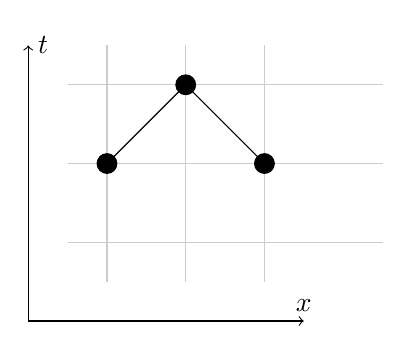
\begin{tikzpicture}
			\draw[<->] (0,3.5) node[right] {\(t\)} -- (0,0) -- (3.5,0) node[above] {\(x\)};
			\draw[white!80!black] (1,0.5) -- (1,3.5);
			\draw[white!80!black] (2,0.5) -- (2,3.5);
			\draw[white!80!black] (3,0.5) -- (3,3.5);
			\draw[white!80!black] (0.5,1) -- (4.5,1);
			\draw[white!80!black] (0.5,2) -- (4.5,2);
			\draw[white!80!black] (0.5,3) -- (4.5,3);
			\filldraw (1,2) circle (.125);
			\filldraw (3,2) circle (.125);
			\filldraw (2,3) circle (.125);
			\draw (1,2) -- (2,3) -- (3,2);
		\end{tikzpicture}
	\end{center}
	\item Let's consider a temporal Taylor expansion of the solution
	\[
		u\parentheses*{x, t + \Delta t} = u\parentheses*{x, t} + \Delta t\partial_t u + \frac{1}{2}\Delta t^2 \partial_{tt}u + \cdots.
	\]
	For the advection equation \(\partial_t u = -a\partial_x u\) we note that the second temporal derivative can be written as
	\[
		\partial_{tt}u = \partial_t \parentheses*{-a\partial_x u} = -a\partial_x \parentheses*{\partial_t u} = a^2 \partial_{xx}u.
	\]
	Hence,
	\[
		u\parentheses*{x, t + \Delta t} \approx u\parentheses*{x, t} - a\Delta t\partial_x u + \frac{a^2}{2}\Delta t^2 \partial_{xx}u
	\]
	and with central finite differences in space we find
	\[
		u_j^{n + 1} = u_j^n + \frac{a\Delta t}{2\Delta x}\parentheses*{u_{j + 1}^n - u_{j + 1}^n} + \frac{a^2 \Delta t^2}{2\Delta x^2}\parentheses*{u_{j - 1}^n - 2u_j + u_{j + 1}^n}.
	\]
	This is the \emph{Lax-Wendroff method}. The stencil is identical to the one of the central method.
	\item An implicit method involving three time levels is given by using both central differences in time and space
	\[
		u_j^{n + 1} = u_j^{n - 1} + \frac{a\Delta t}{\Delta x}\parentheses*{u_{j - 1}^{n + 1} - u_{j + 1}^{n + 1}}.
	\]
	However, in the following we will only consider explicit methods with two time levels, so-called \emph{one-step methods}.
\end{enumerate}
	

\subsection{Error and consistency}

We need to introduce concepts by which we can distinguish the different methods.

\begin{definition}[Error and convergence]
	Let \(u\) be the exact solution of the conservation law and \(u_{\Delta t}\) the numerical approximation as a grid function.
	\begin{enumerate}
		\item The \emph{global error} \(E_{\Delta t}: \R \times \R^+ \to \R\) is defined ny
		\[
			E_{\Delta t}\parentheses*{x, t} := u_{\Delta t}\parentheses*{x, t} - u\parentheses*{x, t}.
		\]
		\item A method is said to be \emph{convergent}, if
		\[
			\norm*{E_{\Delta t}\parentheses*{\cdot, t}} \xrightarrow{\Delta t \to 0} 0
		\]
		for any \(t \in \R^+\) in a suitable norm.
	\end{enumerate}
\end{definition}

\begin{remark}
	\begin{enumerate}
		\item Recall that the grid function \(u_{\Delta t}\) is characterized by both step sizes \(\Delta t\) and \(\Delta x\).
		However, in view of the condition \(\frac{\Delta x}{\Delta t} = \text{const.}\) the limit \(\Delta t \to 0\) implies that \(\Delta x \to 0\) simultaneously.
		Consequently, the convergence definition above is meaningful.
		\item Typical norms are the \(L^1\)-norm and the \(L^\infty\)-norm.
		The use of \(L^2\)-norms are rare in the context of conservation laws.
		\item Essential for convergence are the concepts of consistency and stability.
	\end{enumerate}
\end{remark}

\begin{definition}[Consistency]
	Let \(u\) be the exact solution of a conservation law.
	The \emph{local consistency error} \(L_{\Delta t}: \R \times \R^+ \to \R\) of a time step method \(H_{\Delta t}\) is given by
	\[
		L_{\Delta t}\parentheses*{x, t} = \frac{1}{\Delta t}\parentheses*{u\parentheses*{x, t + \Delta t} - H_{\Delta t}\parentheses*{u\parentheses*{\cdot, t}; x}}.
	\]
	A method \(H_{\Delta t}\) is called
	\begin{enumerate}
		\item \emph{consistent}, if
		\[
			\lim_{\Delta t \to 0}\norm*{L_{\Delta t}\parentheses*{\cdot, t}} = 0 \quad \forall t \in \R^+,
		\]
		\item \emph{consistent of order \(p\)}, if
		\[
			\norm*{L_{\Delta t}\parentheses*{\cdot, t}} \le C\Delta t^p \quad \text{as }\Delta t \to 0
		\]
		for a smooth \(u\) and all \(t \in \R^+\).
	\end{enumerate}
\end{definition}

\begin{remark}
	\begin{enumerate}
		\item The local consistency error assesses the exact solution at time \(t\) and performs a single update with \(H_{\Delta t}\).
		The result is compared with the exact solution at \(t + \Delta t\).
		This is, it is a (local) temporal consistency concept.
		\item For non-smooth solutions we need a different notion of consistency order.
	\end{enumerate}
\end{remark}

\begin{example}[Consistency of Lax-Friedrichs]
	The Lax-Friedrichs method for the advection equation reads
	\[
		u_j^{n + 1} = H_{\Delta t}\parentheses*{u_{\Delta x}^n; j} := \frac{1}{2}\parentheses*{u_{j + 1}^n + u_{j - 1}^n} + \frac{a\Delta t}{2\Delta x}\parentheses*{u_{j - 1}^n - u_{j + 1}^n}.
	\]
	To assess the consistency error we need to consider \(H_{\Delta t}\) applied to the exact solution \(u\parentheses*{\cdot, t}\) and evaluated it at a generic \(x\) instead of \(x_j\).
	That is
	\begin{align*}
		H_{\Delta t}\parentheses*{u\parentheses*{\cdot, t}; x} &\equiv \brackets*{H_{\Delta t}\parentheses*{u\parentheses*{\cdot, t}}}\parentheses*{x}\\
		&= \frac{1}{2}\parentheses*{u\parentheses*{x + \Delta x, t} + u\parentheses*{x - \Delta x, t}} + \frac{a\Delta t}{2\Delta x}\parentheses*{u\parentheses*{x - \Delta x, t} - u\parentheses*{x + \Delta x, t}}.
	\end{align*}
	With some reordering the consistency error thus becomes
	\[
		L_{\Delta t}\parentheses*{x, t} = \frac{1}{\Delta t}\parentheses*{u\parentheses*{x, t + \Delta t} - \parentheses*{\parentheses*{\frac{1}{2} + \frac{a\Delta t}{2\Delta x}}u\parentheses*{x - \Delta x, t} + \parentheses*{\frac{1}{2} - \frac{a\Delta t}{2\Delta x}}u\parentheses*{x + \Delta x, t}}}.
	\]
	Since \(u\) is smooth, we use a Taylor expansion in \(t\) and \(x\) up to third order to find
	\begin{align*}
		u\parentheses*{x, t + \Delta t} &= u\parentheses*{x, t} + \Delta t\partial_t u\parentheses*{x, t} + \frac{1}{2}\Delta t^2 \partial_{tt}u\parentheses*{x, t} + \mathcal{O}\parentheses*{\Delta t^3},\\
		u\parentheses*{x \pm \Delta x, t} &= u\parentheses*{x, t} \pm \Delta x\partial_x u\parentheses*{x, t} + \frac{1}{2}\Delta x^2 \partial_{xx}u\parentheses*{x, t} + \mathcal{O}\parentheses*{\Delta x^3}.
	\end{align*}
	Next we use the advection equation to convert the time derivatives into space derivatives (see also above), that is,
	\[
		\partial_t u = -a\partial_x u \quad \text{and} \quad \partial_{tt} u = a^2 \partial_{xx}u.
	\]
	This gives
	\begin{align*}
		L_{\Delta t}\parentheses*{x, t} &= \frac{1}{\Delta t}\parentheses*{\frac{1}{2}\Delta t^2 a^2 \partial_{xx}u - \parentheses*{\frac{1}{2} + \frac{1}{2}}\frac{1}{2}\Delta x^2 \partial_{xx}u + \mathcal{O}\parentheses*{\Delta t^3} + \mathcal{O}\parentheses*{\Delta x^3}}\\
		&= \frac{\Delta t}{2}\parentheses*{a^2 - \frac{\Delta x^2}{\Delta t^2}}\partial_{xx}u\parentheses*{x, t} + \mathcal{O}\parentheses*{\Delta t^2},
	\end{align*}
	where we have used \(\mathcal{O}\parentheses*{\Delta t} = \mathcal{O}\parentheses*{\Delta x}\) because \(\frac{\Delta x}{\Delta t} = \text{const.}\) by assumption.
	Taking any norm leads to
	\[
		\norm*{L_{\Delta t}\parentheses*{\cdot, t}} \le \frac{1}{2}\absolute*{a^2 - \frac{\Delta x^2}{\Delta t^2}}\norm*{\partial_{xx}u}\Delta t,
	\]
	and hence, the Lax-Friedrichs method is consistent of order \(p = 1\).
\end{example}


\subsection{Stability and convergence}

\begin{definition}[Linear methods]
	A (time step) method \(H_{\Delta t}\) is called \emph{linear}, if it satisfies
	\[
		\alpha H_{\Delta t}\parentheses*{u} + \beta H_{\Delta t}\parentheses*{v} = H_{\Delta t}\parentheses*{\alpha u + \beta v}
	\]
	for any two grid functions \(u, v\) and scalars \(\alpha, \beta \in \R\).
	The one step update of a linear method can then be written as a matrix multiplication:
	\[
		u_{\Delta x}^{n + 1} = H_{\Delta t}u_{\Delta x}^n.
	\]
\end{definition}

\begin{definition}[Stability]
	A linear method \(H_{\Delta t}\) is called \emph{stable} (in the sense of Lax-Richtmyer), if
	\[
		\norm*{u_{\Delta x}^n} = \norm*{H_{\Delta t}^n u_{\Delta x}^0} \le C\norm*{u_{\Delta x}^0}
	\]
	for all \(n \in \N\) with a \(C\) independent of \(\Delta t\).
	Here \(H_{\Delta t}^n \equiv H_{\Delta t}^{\parentheses*{n}} := \parentheses*{H_{\Delta t}}^n\) denotes the \(n\)-fold application of the one step update.
\end{definition}

\begin{remark}
	\begin{enumerate}
		\item All methods that we have considered so far are linear.
		\item For stability it suffices to show that
		\[
			\norm*{H_{\Delta t}u_{\Delta x}} \le \parentheses*{1 + \alpha\Delta t}\norm*{u_{\Delta x}}
		\]
		for any grid vector \(u_{\Delta x}\) and \(\alpha \in \R\), because
		\[
			\norm*{H_{\Delta t}^n u_{\Delta x}} \le \parentheses*{1 + \alpha\Delta t}\norm*{H_{\Delta t}^{n - 1}u_{\Delta x}} \le \parentheses*{1 + \alpha\Delta t}^n \norm*{u_{\Delta x}^0}
		\]
		and
		\[
			\parentheses*{1 + \alpha\Delta t}^n \le e^{\alpha n\Delta t} = e^{\alpha T} = C
		\]
		with \(T = n\Delta t\) the final time.
		Note that this argument only provides a sufficient condition for finite time horizons.
		\item In view of our convention to identify a piecewise constant grid function from the corresponding (grid) vector, stability is defined analogously for grid functions.
		We will thus occasionally use grid functions and grid vectors interchangeably.
		\item Finally, note that stability is norm-dependent.
	\end{enumerate}
\end{remark}

\begin{example}[\(L^1\)-stability of Lax-Friedrichs]
	We consider the Lax-Friedrichs method agian, i.e., the linear method with componentwise one step updates
	\[
		u_j^{n + 1} := H_{\Delta t}\parentheses*{u_{\Delta x}^n; j} = \frac{1}{2}\parentheses*{1 - \frac{a\Delta t}{\Delta x}}u_{j + 1}^n + \frac{1}{2}\parentheses*{1 + \frac{a\Delta t}{\Delta x}}u_{j - 1}^n.
	\]
	Moreover, we study stability with respect to the \(L^1\)-norm, which can be written as (identifying grid vector by its grid function)
	\[
		\norm*{u_{\Delta x}^n}_{L^1\parentheses*{\R}} \equiv \norm*{u_{\Delta t}\parentheses*{\cdot, t_n}}_{L^1\parentheses*{\R}} = \int_\R \absolute*{u_{\Delta t}\parentheses*{x, t_n}}\d x = \Delta x\sum_{j \in \Z}\absolute*{u_j^n},
	\]
	for any grid function \(u_{\Delta t}\) using the compact support.
	Note that we suppress the time level \(n\) here, as we focus on an arbitrary grid function.
	Suppose that \(1 \pm \frac{\alpha\Delta t}{\Delta x} \ge 0\).
	Then we compute
	\begin{align*}
		\norm*{H_{\Delta t}u_{\Delta x}^n}_{L^1\parentheses*{\R}} &= \frac{\Delta x}{2}\sum_{j \in \Z}\absolute*{\parentheses*{1 - \frac{a\Delta t}{\Delta x}}u_{j + 1}^n + \parentheses*{1 + \frac{a\Delta t}{\Delta x}}u_{j - 1}^n}\\
		&\le \frac{\Delta x}{2}\sum_{j \in \Z}\parentheses*{\parentheses*{1 - \frac{a\Delta t}{\Delta x}}\absolute*{u_{j + 1}^n} + \parentheses*{1 + \frac{a\Delta t}{\Delta x}}\absolute*{u_{j - 1}^n}}\\
		&= \frac{1}{2}\parentheses*{1 - \frac{a\Delta t}{\Delta x}}\Delta x\sum_{j \in \Z}\absolute*{u_{j + 1}^n} + \frac{1}{2}\parentheses*{1 + \frac{a\Delta t}{\Delta x}}\Delta x\sum_{j \in \Z}\absolute*{u_{j - 1}^n}\\
		&= \frac{1}{2}\parentheses*{1 - \frac{a\Delta t}{\Delta x}}\norm*{u_{\Delta t}\parentheses*{\cdot, t_n}}_{L^1\parentheses*{\R}} + \frac{1}{2}\parentheses*{1 + \frac{a\Delta t}{\Delta x}}\norm*{u_{\Delta t}\parentheses*{\cdot, t_n}}_{L^1\parentheses*{\R}}\\
		&= \norm*{u_{\Delta t}\parentheses*{\cdot, t_n}}_{L^1\parentheses*{\R}}.
	\end{align*}
	Hence, at least for
	\[
		-1 \le \frac{a\Delta t}{\Delta x} \le 1,
	\]
	the Lax-Friedrichs method is \(L^1\)-stable.
\end{example}

We already know the importance of stability for convergence from finite difference methods.
This is not different here.

\begin{theorem}[Convergence theorem]
	For a consistent, linear method \(H_{\Delta t}\) we have that
	\[
		\text{stability} \iff \text{convergence}.
	\]
	Moreover, if \(H_{\Delta t}\) is consistent of order \(p\) for a smooth solution, and if the initial grid function satisfies
	\[
		\norm*{u_{\Delta x}^0 - u_0} \le C_0 \Delta x^p,
	\]
	then the method is also convergent of order \(p\), in the sense that
	\[
		\norm*{E_{\Delta t}\parentheses*{\cdot, t}} \le C\Delta t^p, \quad \text{as }\Delta t \to 0.
	\]
\end{theorem}

\begin{proof}
	We only proof the statement ``\(\text{stability} \implies \text{convergence}\)'' of the first claim, which is the more relevant statement for our purposes.
	Let \(u\) be the exact solution and \(H_{\Delta t}\) a linear method that is order \(p\) consistent.
	Denote by \(L_{\Delta t}\parentheses*{x, t}\) its local consistency error that satisfies
	\[
		\norm*{L_{\Delta t}\parentheses*{\cdot, t}} \le \hat{C}\Delta t^p.
	\]
	Furthermore, method's stability implies that
	\[
		\norm*{H_{\Delta t}^n u_{\Delta x}} \le \tilde{C}\norm*{u_{\Delta x}}.
	\]
	For the global error at time level \(n + 1\), we compute
	\begin{align*}
		E_{\Delta t}\parentheses*{x, t_{n + 1}} &= u_{\Delta t}\parentheses*{x, t_{n + 1}} - u\parentheses*{x, t_{n + 1}}\\
		&= \brackets*{H_{\Delta t}\parentheses*{u_{\Delta x}\parentheses*{\cdot, t_n}}}\parentheses*{x} - u\parentheses*{x, t_{n + 1}} + \brackets*{H_{\Delta t}\parentheses*{u\parentheses*{\cdot, t_n}}}\parentheses*{x} - \brackets*{H_{\Delta t}\parentheses*{u\parentheses*{\cdot, t_n}}}\parentheses*{x}\\
		&= \brackets*{H_{\Delta t}\parentheses*{u_{\Delta t}\parentheses*{\cdot, t_n} - u\parentheses*{\cdot, t_n}}}\parentheses*{x} - \Delta tL_{\Delta t}\parentheses*{x, t_n},
	\end{align*}
	where we have used the linearity of \(H_{\Delta t}\) and the definition of \(L_{\Delta t}\).
	Identifying the global error \(E_{\Delta t}^{\parentheses*{n}} := E_{\Delta t}\parentheses*{\cdot, t_n}\), we can write the preceding display as
	\[
		E_{\Delta t}^{\parentheses*{n + 1}} = H_{\Delta t}E_{\Delta t}^{\parentheses*{n}} - \Delta t L_{\Delta t}^{\parentheses*{n}},
	\]
	where \(L_{\Delta t}^{\parentheses*{n}} := L_{\Delta t}\parentheses*{\cdot, t_n}\).
	Using this recursively gives
	\[
		E_{\Delta t}^{\parentheses*{n}} = H_{\Delta t}^{\parentheses*{n}}E_{\Delta t}^{\parentheses*{0}} - \Delta t\sum_{i = 1}^n H_{\Delta t}^{\parentheses*{n - i}}L_{\Delta t}^{i - 1}.
	\]
	Employing stability and consistency for \(H_{\Delta t}\) we obtain for the norm
	\begin{align*}
		\norm*{E_{\Delta t}^{\parentheses*{n}}} &\le \norm*{H_{\Delta t}^{\parentheses*{n}}E_{\Delta t}^{\parentheses*{0}}} + \Delta t\sum_{i = 1}^n \norm*{H_{\Delta t}^{\parentheses*{n - i}}L_{\Delta t}^{\parentheses*{i - 1}}}\\
		&\le \tilde{C}\norm*{E_{\Delta t}^{\parentheses*{0}}} + \Delta t\tilde{C}\sum_{i = 1}^n \norm*{L_{\Delta t}^{\parentheses*{i - 1}}}\\
		&\le \tilde{C}\norm*{E_{\Delta t}^{\parentheses*{0}}} + \Delta t\tilde{C}\Delta t^p.
	\end{align*}
	The first term is the discretization of the initial condition and provides the estimate
	\[
		\norm*{E_{\Delta t}^{\parentheses*{0}}} = \norm*{u_{\Delta x}^0 - u_0} \le C_0 \Delta x^p \le \hat{C}_0 \Delta t^p,
	\]
	while the sum generates a factor \(n\) with \(n\Delta t = t_n\) such that
	\[
		\norm*{E_{\Delta t}^{\parentheses*{n}}} \le \tilde{C}\hat{C}_0 \Delta t^p + n\Delta t\tilde{C}\hat{C}\Delta t^p = C\Delta t^p
	\]
\end{proof}

\begin{definition}[Numerical domain of dependence]
	The \emph{numerical domain of dependence} \(D_{\Delta t}\parentheses*{x_i, t_n}\) contains those grid points of the intial time level on which the numerical solution \(u_i^n\) at \(\parentheses*{x_i, t_n}\) may depend, or equivalently, those points that influence \(u_i^n\).
\end{definition}

\begin{theorem}[CFL-condition (Courant-Friedrichs-Levy)]
	For a numerical method to converge to the analytical solution at \(\parentheses*{x, t} \in \R \times \R^+\) it is necessary that
	\[
		D\parentheses*{x, t} \subset \lim_{\Delta t \to 0}D_{\Delta t}\parentheses*{x, t},
	\]
	where \(D\parentheses*{x, t}\) denotes the exact domain of dependence of the solution at \(\parentheses*{x, t}\).
	This is also known as the \emph{CFL-condition}.
\end{theorem}

\begin{proof}
	More or less clear, originally formulated in the context of an existence proof for PDEs.
\end{proof}

\begin{example}[CFL for one-sided methods]
	Let's consider the one-sided method with stencil ``pointing'' to the left, applied to the advection equation with \(a > 0\):
	\[
		u_j^{n + 1} = u_j^n + \frac{a\Delta t}{\Delta x}\parentheses*{u_{j - 1}^n - u_j^n}.
	\]
	The numerical domain of dependence is therefore
	\[
		D_{\Delta t}\parentheses*{x_i, t_n} = \braces*{x_j : -n\Delta x \le x_j - x_i \le 0}.
	\]
	Introducing the \emph{Courant number} \(\nu = \frac{a\Delta t}{\Delta x}\), we can write \(n\Delta x = n\Delta t\frac{\Delta x}{\Delta t} = t_n \frac{a}{\nu}\).
	Hence, the limit of the numerical domain of dependence at a fixed point \(\parentheses*{\bar{x}, \bar{t} \equiv t_n}\) simply is
	\[
		\lim_{\Delta t \to 0}D_{\Delta t}\parentheses*{\bar{x}, \bar{t}} = \braces*{x : -\frac{a\bar{x}}{\nu} \le x - \bar{x} \le 0}.
	\]
	The \emph{analytical} domain of dependence of the advection equation is just a single point
	\[
		D\parentheses*{\bar{x}, \bar{t}} = \braces*{x : x = \bar{x} - a\bar{t}}.
	\]
	The CFL therefore requires that
	\[
		\bar{x} - a\bar{t} \in \braces*{x : -\frac{a\bar{t}}{\nu} \le x - \bar{x} \le 0} \implies -\frac{a\bar{t}}{\nu} \le -a\bar{t} \le 0,
	\]
	which implies that \(0 \le \nu \le 1\).
	Alternatively, this can be stated as \(0 \le \Delta t \le \frac{\Delta x}{a}\), which is a constraint on the time step, in particular for \(a > 0\) we have the picture:
	\begin{center}
		
\begin{tikzpicture}
			\fill[red] (0,0) rectangle (5,5) node[pos=.5] {\emph{TODO}};
		\end{tikzpicture}
	\end{center}
	This discussion also highlights that in order to solve the advection equation with \(a < 0\), the method's stencil has to be turned to point to the right
	\[
		u_j^{n + 1} = u_j^n + \frac{a\Delta t}{\Delta x}\parentheses*{u_j^n - u_{j + 1}^n}.
	\]
	That is, to meet the CFL condition, it is necessary that one-sided methods use stencils that point into the flow.
	The respective methods are called \emph{upwind methods}.
\end{example}

\begin{remark}
	\begin{enumerate}
		\item In fact, any explicit time step method with symmetric stencil including the grid points \(\braces*{u_{j - 1}^n, u_j^n, u_{j + 1}^n}\) will have the CFL-condition
		\[
			\absolute*{\nu} \le 1 \quad \text{or} \quad \Delta t \le \frac{\Delta x}{\absolute*{a}}.
		\]
		However, stability may result in stricter additional conditions.
		\item Implicit methods may have an infinite domain of dependence (the entire grid) and the CFL-condition provides no constraint on \(\Delta t\).
		However a large value of \(\Delta t\) may result in a large consistency error.
	\end{enumerate}
\end{remark}


\subsection{von-Neumann analysis}

To asses stability properties of a numerical method for approximating conservation laws with respect to the \(L^2\)-norm, it is sometimes convenient to use a discrete Fourier transform.
Specifically, we use the complex representation of a \(2\pi\)-periodic
 grid function associated with the discrete values \(u_j^n\) at the nodes \(x_j := \frac{\parentheses*{j - 1}2\pi}{N}, j = 1, \ldots, N\), so that
 \[
 	u_j^n = \sum_{k = 0}^{N - 1}\hat{u}_k^n e^{ikx_j} = \sum_{k = 0}^{N - 1}\hat{u}_k^n e^{\frac{2ik\parentheses*{j - 1}\pi}{N}}, \quad j = 1, \ldots, N,
 \]
 where \(\hat{u}_k^n\) is the amplitude of the \(k\)-th Fourier mode \(x \mapsto e^{ikx}\) at time \(t_n\) for \(k = 0, \ldots, N\).

\begin{theorem}[von-Neumann stability]
	In discrete Fourier space a linear method can be written as an update of the individual amplitudes of the form
	\[
		\hat{u}_k^{n + 1} = g_{\Delta t}\parentheses*{k\Delta x}\hat{u}_k^n, \quad k = 0, \ldots, N - 1,
	\]
	where \(g_{\Delta t}: \R \to \C, \xi \mapsto g_{\Delta t}\parentheses*{\xi}\) is a \(2\pi\)-periodic, complex-valued function, which is called \emph{amplification function}.
	Furthermore, the method is \(L^2\)-norm stable (or \emph{von-Neumann stable}), if
	\[
		\max_{0 \le \xi \le 2\pi}\absolute*{g_{\Delta t}\parentheses*{\xi}} \le 1 + \alpha\Delta t
	\]
	for some \(\alpha \in \R\).
\end{theorem}

\begin{proof}
	Let \(e_k\parentheses*{x} := e^{ikx}\) the \(k\)-th Fourier mode, \(k = 0, \ldots, N - 1\).
	Then
	\[
		u_j^n = \sum_{k = 0}^{N - 1}\hat{u}_k^n e_k\parentheses*{x_j}, \quad j = 1, \ldots, N.
	\]
	Due to the linearity of the discrete Fourier representation it suffices to consider the update of one Fourier mode.
	That is, if \(v_j^n := \hat{u}_k^n e^{ikx_j} \equiv \hat{u}_k^n e_k\parentheses*{x_j}\), then
	\[
		v_j^{n + 1} = \hat{u}_k^{n + 1}e^{ikx_j} = \hat{u}_k^{n + 1}e_k\parentheses*{x_j} = H_{\Delta t}\parentheses*{\hat{u}_k^n e_k; j} = H_{\Delta t}\parentheses*{e_k; j}\hat{u}_k^n,
	\]
	which implies the formal definition
	\[
		g_{\Delta t} = e^{-ikx_j}H_{\Delta t}\parentheses*{e_k; j} = H_{\Delta t}\parentheses*{e^{-ikx_j}; j}
	\]
	for the amplificatino function.
	Because of the shift by the nodes \(x_j\) this expression becomes independent of node \(x_j\) and depends only on the shift \(\xi = k\Delta x\).
	It also follows that \(g\) is \(2\pi\)-periodic and in general complex valued.
	For stability with respect to the \(L^2\)-norm, we use properties of the Fourier transforms to find
	\begin{align*}
		\norm*{u_{\Delta x}^{n + 1}}_2^2 &= N\sum_{k = 0}^{N - 1}\absolute*{\hat{u}_k^{n + 1}}^2\\
		&= N\sum_{k = 0}^{N - 1}\absolute*{g_{\Delta t}\parentheses*{k\Delta x}\hat{u}_k^n}^2\\
		&\le N\max_\xi\absolute*{g_{\Delta t}\parentheses*{\xi}}^2 \sum_{k = 0}^{N - 1}\absolute*{\hat{u}_k^n}^2\\
		&= \max_\xi\absolute*{g_{\Delta t}\parentheses*{\xi}}^2 \norm*{u_{\Delta x}^n}_2^2\\
		&\le \parentheses*{1 + \alpha\Delta t}^2 \norm*{u_{\Delta x}^n}_2^2,
	\end{align*}
	which gives the stability statement
	\[
		\norm*{u_{\Delta x}^{n + 1}}_2 \le \absolute*{1 + \alpha\Delta t}\norm*{u_{\Delta x}^n}_2 \le \parentheses*{1 + \absolute*{\alpha}\Delta t}\norm*{u_{\Delta x}^n}_2,
	\]
	from which the stability in the \(L^2\)-norm follows.
\end{proof}

\begin{example}[von-Neumann stability for the upwind method]
	Let's consider the upwind method
	\[
		u_j^{n + 1} = u_j^n + \frac{a\Delta t}{\Delta x}\parentheses*{u*{i - 1}^n - u_i^n} = \parentheses*{1 - \nu}u_j^n + \nu u_{j - 1}^n =: H_{\Delta t}\parentheses*{u_{\Delta x}^n; j}
	\]
	for \(a > 0\) and with Courant number \(\nu = \frac{a\Delta t}{\Delta x}\).
	Inserting a single Fourier mode \(e_k\) at \(x_j\), that is,
	\[
		u_j^n = e^{ikx_j} \equiv e_k\parentheses*{x_j},
	\]
	we obtain
	\begin{align*}
		H_{\Delta t}\parentheses*{e_k; j} &\equiv H_{\Delta t}\parentheses*{e^{ik\parentheses*{\cdot}}; j}\\
		&= \parentheses*{1 - \nu}e^{ikx_j} + \nu e^{ik\parentheses*{x_j - \Delta x}}\\
		&= \parentheses*{\parentheses*{1 - \nu} + \nu e^{-ik\Delta x}}e^{ikx_j},
	\end{align*}
	which thus gives
	\[
		g_{\Delta t}\parentheses*{\xi} = \parentheses*{1 - \nu} + \nu e^{-i\xi} = 1 - \nu\parentheses*{1 - \cos\xi} - i\nu\sin\xi.
	\]
	Due to periodicity this function gives closed lines in the imaginary plane.
	A plot for varying values of \(\nu\) looks like this:
	\begin{center}
		
\begin{tikzpicture}
			\fill[red] (0,0) rectangle (5,5) node[pos=.5] {\emph{TODO}};
		\end{tikzpicture}
	\end{center}
	From detailed investigations we conclude that
	\[
		\absolute*{g\parentheses*{\xi}} \le 1 \iff 0 \le \nu \le 1,
	\]
	which corresponds to the CFL condition.
\end{example}


\subsection{Discontionuous solutions}

The order of consistency indicates the quality of approximation for smooth solutions.
For discontinuous solutions the approximation accuracy is therefore not clear.
As a matter of fact, it is not even clear how to measure approximation quality.
We begin with the following idea.

\begin{definition}[High-resolution schemes]
	If a numerical methods represents discontinuities in a ``good way'', that is, with sharp gradients and without oscillations, it is called a \emph{high-resolution method}.
\end{definition}

The methods that we have considered so far provide very different results for discontinuous solutions.
The question thus is:
How can we understand these shapes?

\begin{definition}[Modified equation]
	Consider a method that is consistent of order \(p > 0\).
	Suppose that the local (consistency) error \(L_{\Delta t}\) has the representation
	\[
		L_{\Delta t}\parentheses*{x, t} = \Delta t^p \mathcal{L}_{\Delta t}^{\parentheses*{p}}\brackets*{u}\parentheses*{x, t} + \mathcal{O}\parentheses*{\Delta t^{p + 1}}
	\]
	for the advection equation with solution \(u\).
	Here, \(\mathcal{L}_{\Delta t}^{\parentheses*{p}}\) is a suitable (spatial) differential operator.
	Then the equation
	\[
		\partial_t u + a\partial_x u = -\Delta t^p \mathcal{L}_{\Delta t}^{\parentheses*{p}}\brackets*{u}
	\]
	is called \emph{modified equation} for the advection equation.
\end{definition}

\begin{remark}
	\begin{enumerate}
		\item For Lax-Friedrichs we have seen earlier that
		\[
			L_{\Delta t}\parentheses*{x, t} = \frac{\Delta t}{2}\parentheses*{a^2 - \frac{\Delta x^2}{\Delta t^2}}\partial_{xx}u\parentheses*{x, t} + \mathcal{O}\parentheses*{\Delta t^2},
		\]
		so that the sought-after differential operator is essentially a second order derivative
		\[
			\mathcal{L}_{\Delta t}^{\parentheses*{p}}\brackets*{u} = \frac{1}{2}\parentheses*{a^2 - \frac{\Delta x^2}{\Delta t^2}}\partial_{xx}u.
		\]
		In general, a \(p\)-th order method will be associated with a differential ooperatr of \(p + 1\)-order in the modified equation.
		\item The modified equation provides an analytical tool to understand the shape of the numerical solution.
		Notice that this bears similarities to viscosity solutions.
	\end{enumerate}
\end{remark}

\begin{theorem}[Modified equation]
	The (numerical) result obtained from a consistent method with order \(p \ge 1\) for the advection equation, is a consistent approximation of the solution to its corresponding modified equation with order \(p + 1\).
\end{theorem}

\begin{proof}
	We consider the local (consistency) error
	\[
		L_{\Delta t}\parentheses*{x, t} = \frac{1}{\Delta t}\parentheses*{u\parentheses*{x, t + \Delta t} - H_{\Delta t}\parentheses*{u\parentheses*{\cdot, t}; x}},
	\]
	where \(u\) satisfies the advection equation, and use a Taylor expansion for each term:
	\begin{align*}
		H_{\Delta t}\parentheses*{u\parentheses*{\cdot, t}; x} &= \sum_{n = 0}^{p + 1}\alpha_n \Delta x^n \partial_x^{\parentheses*{n}}u\parentheses*{x, t} + \mathcal{O}\parentheses*{\Delta x^{p + 2}},\\
		u\parentheses*{x, t + \Delta t} &= \sum_{n = 0}^{p + 1}\frac{1}{n!}\Delta t^n \partial_t^{\parentheses*{n}}u\parentheses*{x, t} + \mathcal{O}\parentheses*{\Delta t^{p + 2}}.
	\end{align*}
	Here the coefficients \(\alpha_n\) follow from the particular numerical method \(H_{\Delta t}\).
	Taking advantage of the advection equation, specifically the fact that \(\partial_t^n u = \parentheses*{-a}^n \partial_x^n u\), we can replace time derivatives by spatial derivatives and obtain
	\[
		\Delta tL_{\Delta t}\parentheses*{x, t} = \sum_{n = 0}^{p + 1}\parentheses*{\frac{\parentheses*{-a}^n}{n!}\Delta t^n - \alpha_n \Delta x^n}\partial_x^{\parentheses*{n}}u\parentheses*{x, t} + \mathcal{O}\parentheses*{\Delta x^{p + 2}}.
	\]
	Because the method is order \(p\) consistent, it follows that the coefficient \(\alpha_n\) are such that the terms in parentheses multiplying the \(n\)-th spatial derivatives vanish for all \(n\) up to and including \(p\).
	The last term of the sum then defines the differential operator for the modified equation.
	Specifically, let
	\[
		\mathcal{L}_{\Delta t}^{\parentheses*{p}}\brackets*{u} := \parentheses*{\frac{\parentheses*{-a}^{p + 1}}{\parentheses*{p + 1}!} + \alpha_{p + 1}\frac{\Delta x^{p + 1}}{\Delta t^{p + 1}}}\partial_x^{p + 1}u,
	\]
	then we can write the local error as
	\[
		\Delta tL_{\Delta t}\parentheses*{x, t} = \Delta t^{p + 1}\parentheses*{\mathcal{L}_{\Delta t}^{\parentheses*{p}}\brackets*{u}}\parentheses*{x, t} + \mathcal{O}\parentheses*{\Delta t^{p + 2}}.
	\]
	Suppose that \(v\) is the solution of the modified equation \(\partial_t v + a\partial_x v = -\Delta t^p \mathcal{L}_{\Delta t}^{\parentheses*{p}}\brackets*{v}\) associated with the advection equation.
	Then the difference satisfies
	\begin{align*}
		\partial_t \parentheses*{v - u} &= -a\partial_x \parentheses*{v - u} - \Delta t^p \mathcal{L}_{\Delta t}^{\parentheses*{p}}\brackets*{v}\\
		\iff \partial_t^{\parentheses*{n}}\parentheses*{v - u} &= \parentheses*{-a}^n \partial_x^n \parentheses*{u - v} + \mathcal{O}\parentheses*{\Delta t^p} \quad \parentheses*{n \ge 2}.
	\end{align*}
	The local consistency error of \(H_{\Delta t}\parentheses*{u\parentheses*{\cdot, t}}\) as an approximation for \(v\parentheses*{\cdot, t + \Delta t}\) then is
	\begin{align*}
		\frac{v\parentheses*{x, t + \Delta t} - H_{\Delta t}\parentheses*{u\parentheses*{\cdot, t}; x}}{\Delta t} &= L_{\Delta t}\parentheses*{x, t} + \frac{v\parentheses*{x, t + \Delta t} - u\parentheses*{x, t + \Delta t}}{\Delta t}\\
		&= \Delta t^p \mathcal{L}_{\Delta t}^{\parentheses*{p}}\brackets*{u} + \frac{v\parentheses*{x, t + \Delta t}- u\parentheses*{x, t + \Delta t}}{\Delta t} + \mathcal{O}\parentheses*{\Delta t^{p + 1}}.
	\end{align*}
	As consistency assesses the accuracy of an one step update, we can require that \(v\parentheses*{\cdot, t} = u\parentheses*{\cdot, t}\) at time \(t\).
	A Taylor expansion of the difference combined with the transformations between spatial and temporal derivatives eventually yields
	\begin{align*}
		v\parentheses*{x, t + \Delta t} - u\parentheses*{x, t + \Delta t} &= \sum_{n = 0}^{p + 1}\frac{1}{n!}\Delta t^n \partial_t^{\parentheses*{n}}\parentheses*{v\parentheses*{x, t} - u\parentheses*{x, t}} + \mathcal{O}\parentheses*{\Delta t^{p + 2}}\\
		&= -a\Delta t\partial_x \parentheses*{v - u} - \Delta t^{p + 1}\mathcal{L}_{\Delta t}^{\parentheses*{p}}\brackets*{v} + \sum_{n = 2}^{p + 1}\frac{\parentheses*{-a}^n}{n!}\Delta t^n \partial_x^{\parentheses*{n}}\parentheses*{v\parentheses*{x, t} - u\parentheses*{x, t}} + \mathcal{O}\parentheses*{\Delta t^{p + 2}}\\
		&= -\Delta t^{p + 1}\mathcal{L}_{\Delta t}^{\parentheses*{p}}\brackets*{u} + \mathcal{O}\parentheses*{\Delta t^{p + 2}}.
	\end{align*}
	Consequently, we find
	\[
		\frac{v\parentheses*{x, t + \Delta t} - H_{\Delta t}\parentheses*{u\parentheses*{\cdot, t}; x}}{\Delta t} = \mathcal{O}\parentheses*{\Delta t^{p + 1}},
	\]
	as claimed.
\end{proof}

\begin{definition}[Diffusive/dispersive methods]
	Consider the advection equation.
	\begin{enumerate}
		\item Methods of order \(p = 1\) typically have a modified equation of the form
		\[
			\partial_t u + a\partial_x u = D\partial_{xx}u
		\]
		with \(D = \mathcal{O}\parentheses*{\Delta t}\) and are called \emph{diffusive methods}.
		\item Methofs of order \(p = 2\) typically have a modified equation of the form
		\[
			\partial_t u + a\partial_x u = \lambda\partial_{xxx}u
		\]
		with \(\lambda = \mathcal{O}\parentheses*{\Delta t^2}\) and are called \emph{disperive methods}.
	\end{enumerate}
\end{definition}

\begin{remark}
	\begin{enumerate}
		\item The solution of the modified equation describes the approximate behavior of the numerical method more accurately than ``just'' advection.
		\item The modified equation can, for example, be solved by Fourier transform.
		The additional differential operator for diffusive methods corresponds to diffusion and will thus introduce damping of the Fourier modes.
		Motice that the method is unstable for \(D < 0\).
		Similarly, dispersion will propagate the modes with the wrong speed.
	\end{enumerate}
\end{remark}

\begin{example}[Diffusive/dispersive methods]
	For upwind and Lax-Friedrich (LF) methods the wave package has passed through the dimain one time at \(t = 1\) and the result show strong damping.
	For Lax-Wendroff (LW) the wave package has passed through the domain four times at \(t = 4\) and much less damping is present.
	However dispersion (shift of profile) is visible.
	The central method is unstable already at \(t = 0.1\).
\end{example}
